\documentclass[a4paper]{article}
\usepackage{amsfonts}
\usepackage{amsmath}
\usepackage{amssymb}
\usepackage{graphicx}
\newcommand{\bint}{\displaystyle\int\limits}

\begin{document}
  
\noindent \large Auteur: CouldBeMathijs \\
\noindent \large Studierichting: Informatica\\
\noindent \large Oefeningenreeks 5M nr. 2\\

\medskip

\normalsize

$x(t) = a \cdot \cos^3t$ met $a \in \mathbb{R}_0^+ \Rightarrow x'(t)= -3a \cos^2t \sin t$\\

$y(t) = a \cdot \sin^3t \Rightarrow y'(t)= 3a \sin^2t \cos t$\\

Schets:\\

\begin{figure}[h]
\centering
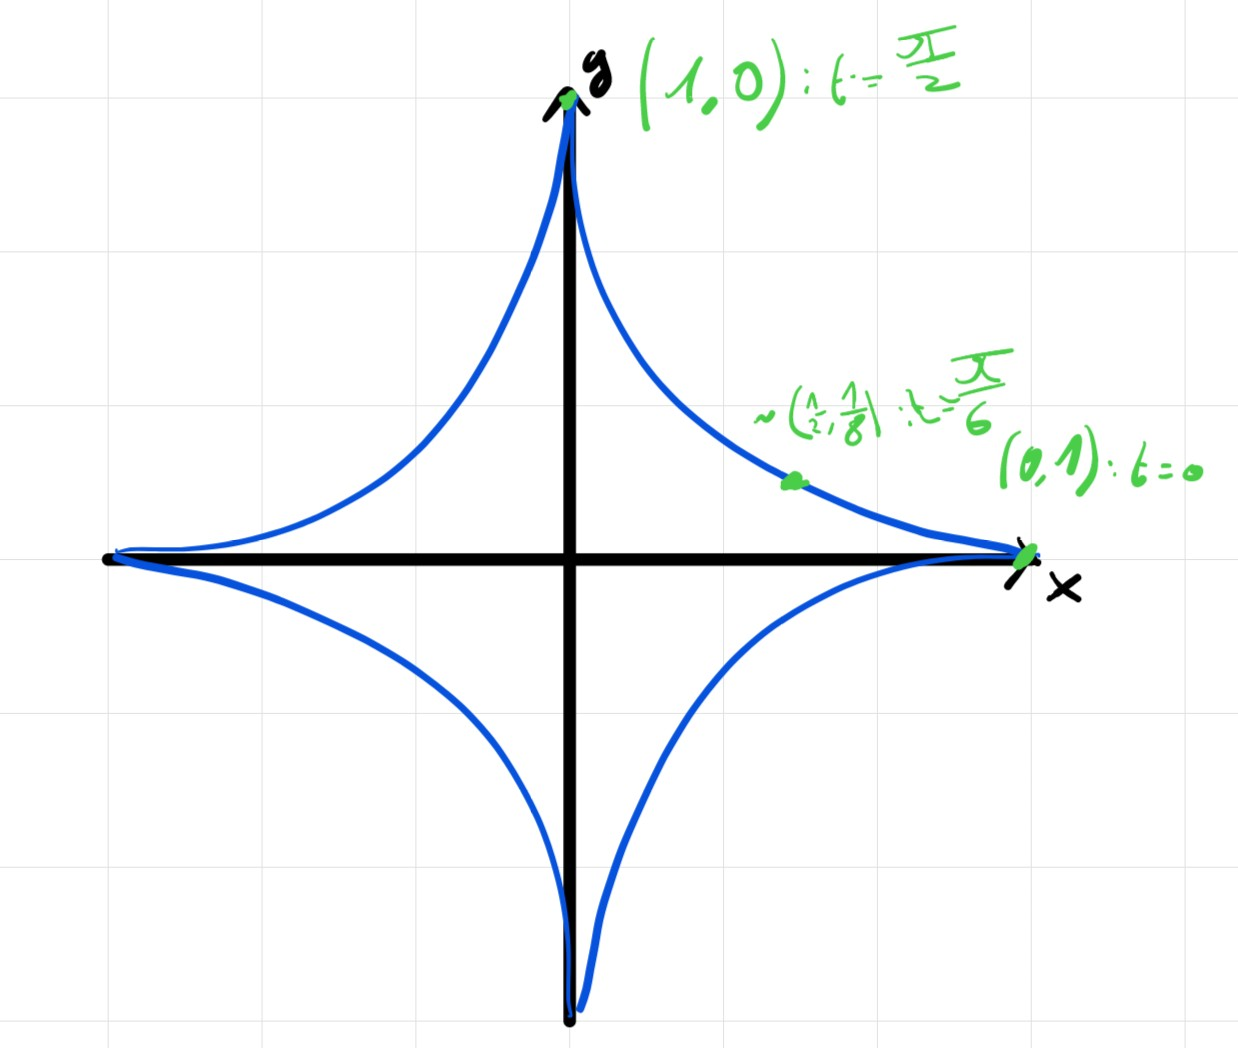
\includegraphics[width=10cm]{5M-2-could.be.mathijs.INF.jpg}
\end{figure}

Van $\dfrac{\pi}{2}$ tot $0$ beschrijft maar een vierde van de oppervlakte,\\

we doen de formule dus maal 4\\

\begin{eqnarray*}
S &=& 4 \pi \bint_{\tfrac{\pi}{2}}^0 |a\cdot\sin^3t| \sqrt{\left(-3a\cos^2t\sin t\right)^2\left(3a\sin^2t\cos t\right)^2}dt\\
&=& 4 \pi \bint_{\tfrac{\pi}{2}}^0 \underbrace{a \cdot \sin^3 t}_{\text{steeds positief}} \cdot 3a \cdot \sqrt{(\cos^2t+\sin^2t)(\cos^2t\sin^2t)}dt\\
&=& 4 \pi \bint_{\tfrac{\pi}{2}}^0 3a^2 \cdot \sin^3 t \cdot \sqrt{1 \cdot (\cos^2t\sin^2t)}dt\\
&=& 12 \pi a^2 \bint_{\tfrac{\pi}{2}}^0 \sin^4t \cos t dt\\
\end{eqnarray*}

Onbepaalde integraal uitwerken:\\

$\bint \sin^4t \cos t dt = \bint \sin^4 t d(\sin t) = \dfrac{\sin^5}{5} + C$ met $C \in \mathbb{R}$\\

$S= 12\pi a^2 \left[\dfrac{\sin^5t}{5}\right]_{\tfrac{\pi}{2}}^0 = \dfrac{-12 \pi a^2}{5}$\\

Antwoord negatief $\Rightarrow$ kies negatieve wortel
$$S = \dfrac{12 \pi a^2}{5}$$


\begin{thebibliography}{999}
%\bibitem{a} Referentie
\end{thebibliography}
\end{document} 
